\section{Evaluations}
\label{sec:main_results}

\subsection{Prompting \& Few-Shot}
\label{sec:prompt_and_fewshot}

We evaluate our model on 16 standard NLP tasks utilized in the literature: HellaSwag \cite{hellaswag}, StoryCloze \cite{storycloze}, PIQA \cite{bisk2020piqa}, ARC Easy and Challenge \cite{arc_challenge}, OpenBookQA \cite{openbookqa}, WinoGrad \cite{levesque2011winograd}, WinoGrande \cite{winogrande}, and SuperGLUE \cite{wang2019superglue}. We follow GPT-3 \cite{brown2020gpt3} by using their prompts and overall experimental setup. We compare primarily to GPT-3, having aimed to re-implement their  evaluation settings, but include reported performance of other LLMs on a per-task basis when available \cite{J1WhitePaper,gopher2022,chinchilla2022,eleutherai2022}

We report performance in accuracy (omitting F1 for MultiRC and ReCoRD for consistency in evaluation metrics). For the Winograd Schema Challenge (WSC) task in the SuperGLUE benchmark, we follow \cite{brown2020gpt3} and formulate the task as multiple choice questions, which is known to affect performance \cite{liu2020precise}.

\paragraph{Zero-shot} Overall average zero-shot performance across all 14 tasks may be seen in Figure~\ref{fig:zeroshot}. Overall, we see our average performance follows the trend of GPT-3. However, performance can vary radically across the tasks: for a full breakdown, see Appendix~\ref{app:full_evals}.  Note that we intentionally removed MultiRC and WIC from these averages, as these datasets seem to systematically favor GPT-3 or OPT disproportionately.

Our performance roughly matched GPT-3 for 10 tasks, and underperformed in 3 tasks (ARC Challenge and MultiRC). In 3 tasks (CB, BoolQ, WSC), we find both GPT and OPT models display unpredictable behavior with respect to scale, likely due to the small size of the validation set in these 3 tasks (56, 277, and 104 examples, respectively). In WIC, we see that the OPT models always outperform the GPT-3 models, though the numbers reported by \citet{brown2020gpt3} also seem questionable, given WIC being a binary classification task.\footnote{\citet{brown2020gpt3} reports 0\% accuracy on WIC, which implies 100\% accuracy if the classification was inverted.} For MultiRC, we are unable to replicate the GPT-3 results using the \davinci{} API\footnote{\url{https://beta.openai.com/docs/engines/overview}} within our evaluation setup, suggesting differences in the methods of evaluation on this task. For BoolQ and WSC, we note that both OPT and GPT models seem to hover around majority-class accuracy, suggesting small perturbations in probability masses may be dominating the evaluations.

Chinchilla \cite{chinchilla2022} and Gopher \cite{gopher2022} perform roughly consistently with others for their parameter sizes, while PaLM \cite{palm2022} generally performs better across all settings, even when controlling for number of parameters. We speculate the high performance of PaLM comes predominantly from higher quality and diversity of pre-training data.


\begin{figure}
    \centering
    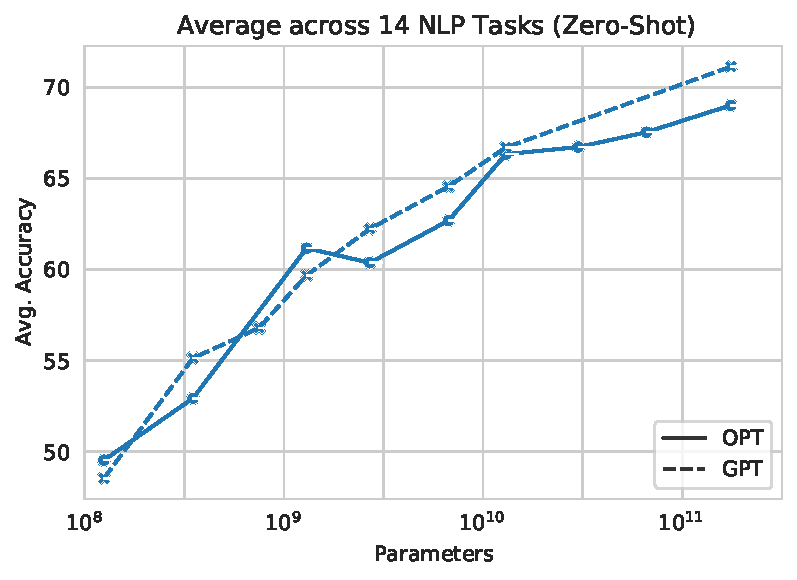
\includegraphics[width=0.98\linewidth]{figures/nlpavg.pdf}
    \caption{{\bf Zero-shot NLP Evaluation Averages}. Across a variety of tasks and model sizes, OPT largely matches the reported averages of GPT-3. However, performance varies greatly per task: see Appendix~\ref{app:full_evals}.}
    \label{fig:zeroshot}
\end{figure}

\begin{figure}[t]
    \centering
    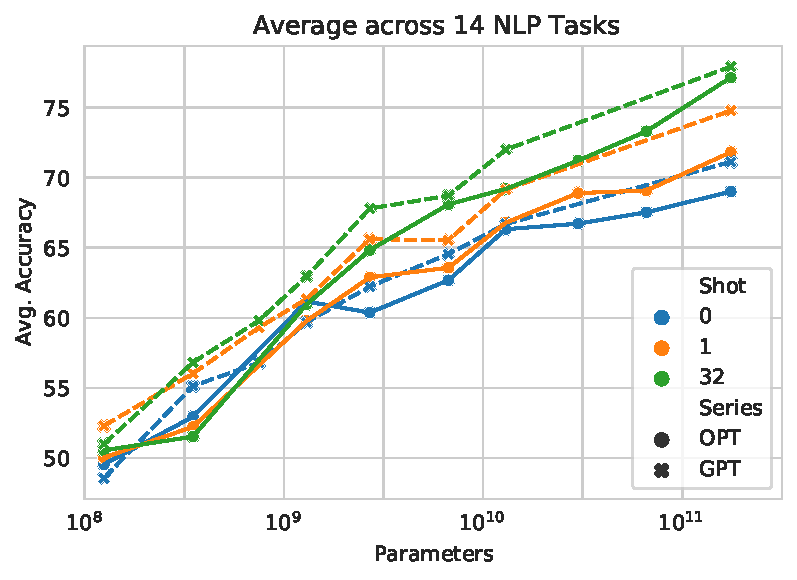
\includegraphics[width=0.98\linewidth]{figures/multishot_avg.pdf}
    \caption{\textbf{Multi-shot performance}. OPT performance for one- and few-shot lags behind GPT-3 models, but performance depends heavily per task; see Appendix~\ref{app:full_evals}.}
    \label{fig:multishot}
\end{figure}

\paragraph{One-shot and Few-shot} Average multi-shot in-context performance is shown in Figure~\ref{fig:multishot} (again, omitting MultiRC and WIC), with detailed performances shown in Appendix~\ref{app:full_evals}. Across the average of all metrics, we find that OPT models perform similarly to GPT-3 models. However, as with zero-shot, breaking down these results per task shows a different story: in the same set of 10 datasets as zero-shot, we see similar performance across the two models. Some of the remaining datasets show inconsistent performance with respect to model size for both OPT and GPT-3 models (BoolQ, CB, WSC, RTE). In MultiRC, we consistently see underperformance of OPT models compared to GPT-3 models. Similar to our zero-shot evaluation, we hypothesize our one- and few-shot evaluation setup may differ significantly from \citet{brown2020gpt3}.

\subsection{Dialogue}
\label{sec:dialogue}

Given that LLMs are known to be an integral component of modern dialogue models \cite{adiwardana2020meena,roller-etal-2021-recipes,thoppilan2022lamda,gopher2022,palm2022}, we additionally evaluate \OPT{} on several open source dialogue datasets. In particular, we follow \citet{roller-etal-2021-recipes}, and evaluate on ConvAI2 \cite{dinan2019second}, Wizard of Wikipedia \cite{dinan2018wizard}, Empathetic Dialogues \cite{rashkin2019empathetic}, and Blended Skill Talk \cite{smith2020bst}. We additionally evaluate on the more recent Wizard of Internet dataset \cite{komeili2021woi}.
We focus our comparisons primarily against existing open source dialogue models including the fine-tuned BlenderBot~1 \cite{roller-etal-2021-recipes} and its pre-training counterpart Reddit 2.7B. We also compare against the fine-tuned R2C2 BlenderBot, a 2.7B parameter BlenderBot-like model trained by \citet{shuster2022language}.

We report Perplexity and Unigram F1 (UF1) overlap, following the metrics of the ConvAI2 competition \cite{dinan2019second}. To control for different tokenization in each of the models, we normalize all perplexities to be in the space of the GPT-2 tokenizer \cite{radford2019language}. We also note which models are supervised with respect to these dialogue tasks and which are unsupervised. For \OPT{}, all generations are performed using greedy decoding up to a maximum of 32 tokens. We do not attempt to prompt the model at all except for alternating ``Person 1:'' and ``Person 2:'' lines of dialogue. The remaining models use the generation parameters found in BlenderBot~1.

\begin{table*}[t]
    \centering
    \begin{tabular}{llrrrrrrrrrr}
    \toprule
    & & \multicolumn{5}{c}{Perplexity ($\downarrow$)} & \multicolumn{5}{c}{Unigram F1 ($\uparrow$)}\\
    \cmidrule(lr){3-7} \cmidrule(lr){8-12}
    {\bf Model} & {\bf Eval} & {\bf C2} & {\bf WW} & {\bf ED} & {\bf BST} & {\bf WoI} & {\bf C2} & {\bf WW} & {\bf ED} & {\bf BST} & {\bf WoI}\\
    \midrule
         Reddit 2.7B             & Unsup. &  18.9  &    21.0 & 11.6   & 17.4    & 18.0   & .126 & .133 & .135 & .133 & .124 \\
         BlenderBot 1            & Sup.   &{\bf10.2}  &    12.5 &{\bf9.0}& 11.9    & 14.7   & .183 & .189 & .192 & .178 & .154\\
         R2C2 BlenderBot             & Sup.   &  10.5  &   {\bf 12.4} &  9.1   &{\bf11.7}& 14.6   &{\bf.205}&{\bf.198}&{\bf.197}&{\bf.186}&{\bf.160}\\
         \tablewhitespace
         \OPT                    & Unsup. &  10.8 & 13.3 & 10.3  &  12.1 & {\bf 12.0} & .185 & .152 & .149 & .162 & .147\\
    \bottomrule
    \end{tabular}
    \caption{{\bf Dialogue Evaluations.} OPT-175B, in a fully unsupervised setting, performs competitively against fully supervised models.}
    \label{tab:dialogue_evals}
\end{table*}

Results are shown in Table~\ref{tab:dialogue_evals}. We see that \OPT{} significantly outperforms the also-unsupervised Reddit 2.7B model on all tasks, and performs competitively with the fully supervised BlenderBot~1 model, especially in the ConvAI2 dataset. On the Wizard-of-Internet dataset, which is fully unsupervised for all models, we see that \OPT{} obtains the lowest perplexity but still has lower UF1 than the models with Wizard-of-Wikipedia supervision.

We were somewhat surprised that the evaluations of the unsupervised \OPT{} model were as competitive as BlenderBot~1 on the ConvAI2 dataset. This may indicate leakage of the ConvAI2 dataset into the general pre-training corpus or even into the validation data as evaluated in Table~\ref{tab:dialogue_evals}. To address concerns of leakage, we searched our pre-training corpus for the first conversation in the ConvAI2 dataset, but we did not find any overlap.
We additionally evaluated \OPT{} on the ConvAI2 hidden test set, which has never been publicly released, and achieved 10.7 ppl and .185 UF1, matching the performance of the validation set. Furthermore, we evaluated \OPT{} on a subset of the ConvAI2-like MultiSessionChat (MSC) dataset \cite{xu2021beyond} and obtained a perplexity of 9.7 and UF1 of .177, indicating the model is generalizing well across multiple PersonaChat-like datasets. Since both MSC and WoI datasets were released \textit{after} the CommonCrawl snapshot used in pre-training corpus, there is minimal risk of leakage. We conclude that \OPT{} has a strong ability to maintain a consistent persona across conversations, a behavior also highlighted in LaMDA \cite{thoppilan2022lamda}.

